\documentclass[12pt]{scrartcl}


\usepackage{hyperref}
\usepackage[pdftex,dvipsnames,cmyk]{xcolor}  % Coloured text etc.
\usepackage{upquote}
\usepackage{url}
\usepackage{appendix}
\usepackage{ifpdf}
\usepackage{placeins}
\ifpdf
  \usepackage[pdftex]{graphicx}
  \graphicspath{{graphics/}}
  \DeclareGraphicsExtensions{.pdf,.jpeg,.jpg,.png}
\else
  \usepackage[dvips]{graphicx}
  \graphicspath{{graphics/}}
  \DeclareGraphicsExtensions{.eps}
\fi

\usepackage[backend=biber,
            bibencoding=utf8,
            natbib=true,
            style=authoryear,
            hyperref=true,
            url=false,
            doi=false,
%            backref=true,
            maxcitenames=3,
            block=ragged]{biblatex}
\addbibresource{refs/thesisbibliointerimreport.bib}

\usepackage[colorinlistoftodos]{todonotes} % remove draft option in \documentclass to disable this package

\usepackage{listings}
\definecolor{pale-gray}{gray}{0.95}
\lstset{backgroundcolor=\color{pale-gray},language=SQL}
\usepackage{caption}
\captionsetup[lstlisting]{labelfont=bf}

\usepackage{minted}
\usemintedstyle{colorful}
\setminted[sql]{frame=lines, framesep=2mm, baselinestretch=1.2, fontsize=\footnotesize, linenos}
\setminted[python]{frame=lines, framesep=2mm, baselinestretch=1.2, fontsize=\footnotesize, linenos}

% See https://texfaq.org/FAQ-casechange
\usepackage[overload]{textcase}


\usepackage[toc]{glossaries}
\usepackage[utf8]{inputenc}
\makeglossaries

\newglossaryentry{Real}
{
    name=Real Energy Consumption,
    description={real power is the actual power consumed by the equipment to do useful work. It is distinguished from apparent power by eliminating the reactive power component that may be present}
}

\newglossaryentry{Reactive}
{
    name=Reactive Energy Consumption,
    description={reactive power \ldots}
}

\newglossaryentry{Apparent}
{
    name=Apparent Energy Consumption,
    description={The combination of reactive power and real power is called apparent power, and it is the product of a circuit's voltage and current, without reference to phase angle. Apparent power is measured in the unit of Volt-Amps (VA) and is symbolized by the capital letter S}
}

\newglossaryentry{Power}
{
    name=Power Factor,
    description={Power Factor (PF) is the ratio between 0 and 1 of real power (kW) to apparent power (kVA)}
}

\newglossaryentry{LCP}
{
    name=LCP Cooling Capacity,
    description={The capacity of the Liquid Cooling Package to cool a rack in a Data Centre(LCP}
}


\begin{document}

\begin{titlepage}
	\newcommand{\HRule}{\rule{\linewidth}{0.5mm}}

	\center
	\textsc{\LARGE Waterford Institute of Technology}\\[1.5cm]
	\HRule\\[0.4cm]

	\huge\bfseries \MakeTextUppercase{Applying Data Mining Techniques to Monitoring Data from a Data Centre to Improve its Energy Efficiency}\\[0.4cm]

	\HRule\\[1.0cm]
	\textsc{\large Interim Report}\\[1.5cm]
	\begin{minipage}{0.4\textwidth}
		\begin{flushleft}
			\large
			\textit{Student}\\
			John Fitzpatrick, 02323826
		\end{flushleft}
	\end{minipage}
	~
	\begin{minipage}{0.4\textwidth}
		\begin{flushright}
			\large
			\textit{Supervisor}\\
      Dr. Bernard Butler
		\end{flushright}
	\end{minipage}


	\vfill\vfill\vfill

	{\large\today}

	\vfill

\end{titlepage}

\newpage
\pagenumbering{roman}
\tableofcontents
\newpage
\listoffigures
\newpage
\lstlistoflistings % needs the listings package
\newpage
\renewcommand\listoflistingscaption{List of source codes}
\listoflistings % needs the inbuilt listings environment of LaTeX; comment out the listings package stuff above otherwise nothing appears here
\newpage
\pagenumbering{arabic}

%\begin{document}

%\title{Thesis Proposal - Title TBC}
%\author{John Fitzpatrick}

%\maketitle

%\pagebreak



\section{Introduction}
\label{sec:[introduction]}
The demand for cloud computing services is growing exponentially, driven by the growth of internet users and applications (\cite{edssch.qt9c84f49g20130101}). As a result, within the Information and Communications Technology sector (ICT), Data Centres are the fastest growing sector in terms of energy consumption and are now responsible for over 2\% of the global CO2 emissions (\cite{edsbas.13818AC20170101}). With this growth in Data Centre energy consumption over the last 10 years, there arises a cost incentive, along with a general green incentive, to reduce energy consumption or to use energy more efficiently. While there is ample literature available that deals with making Data Centres more efficient by changing the hardware configuration of the Data Centre, this Interim Report documents the progress made on applying Data Mining techniques to the monitoring data, compiled from within a Data Centre, to unlock hidden information to assist system administrators to make the Data Centre more efficient. Data from a medium sized Data Centre, the WIT-TSSG Data Centre in the Carriganore West Campus of Waterford institute of Technology is being used for this project.  


\subsection{Motivation}
\label{subsec:[Motivation]}
The goal behind making Data Centres more energy efficient is to reduce the energy consumption while delivering the same service to its users. Therefore the motivation that follows from this is twofold. 

Firstly, there is the motivation to make the Data Centre more energy efficient for the tangible benefits this brings. If energy consumption is reduced, this will lead to cost savings, while simultaneously reducing the carbon footprint of the Data Centre. Ultimately, this could deliver savings to WIT, allowing for potential investment in other educational projects while helping the environment at the same time. 

Secondly, in addition to the overarching motivation above, this research is being motivated by a desire to explore Data Mining techniques to gain insight into Data Centre energy consumption to help make them more energy efficient. While Data Centres are a part component of any cloud computing architecture, the emphasis here is to treat them as an entity in their own right, and use the vast amounts of monitoring data they generate to make them more energy efficient. There is very little existing literature in this regard and the motivation here is that this study would contribute to the research in this field.  

\subsection{Research Problem Statement}
\label{subsec:[Research Problem Statement]}
As outlined in the introduction (section \ref{sec:[introduction]}), The information and Communication Technology (ICT) sector, and Data Centres in particular, are consuming vast amounts of energy and are contributing to an ever increasing carbon footprint.  \citet{edsbas.13818AC20170101} highlight that the ICT sector will consume 13\% of the global electricity supply by 2030. 

Therefore, as the energy demand of Data Centres grows due to the changing role of technology in society, this represents a clear challenge to policymakers, researchers and Data Centre stakeholders to seek solutions to make Data Centres more efficient in terms of energy consumption. 

A significant amount of research exists that focuses on making Data Centres more efficient, by concentrating on improvements to the physical hardware and infrastructure within a Data Centre. This, as detailed in the literature review, (section \ref{subsec:[Improving Data Centre Energy Efficiency]}) specifically focused on such measures as: 

\begin{enumerate}
	\item Introducing wireless sensors to capture key metrics;
	\item Following best practices and 
	\item Focussing on specific features within a Data Centre to gain efficiencies, such as the cooling system, server efficiencies, network modelling, or the optimisation of applications at an infrastructural level. 
\end{enumerate}

However, this research has a different focus. It analyses existing monitoring data, that is already stored by the Data Centre to seek hidden insights that might make a Data Centre more energy efficient. 

\subsection{Aims and Objectives}
\label{subsec:[Aims and Objective]}

The ultimate aim of this research, as specified in the Research Problem Statement (section \ref{subsec:[Research Problem Statement]}) is to use Data Mining Techniques on the monitoring data compiled at the WIT-TSSG Data Centre to gain hidden insights about energy consumption to help make the Data Centre more energy efficient. 
Specifically, the following are the aims and objectives of the project:

\begin{itemize}
\item Review all existing literature on improving Data Centre energy efficiency.
\item Learn about the WIT-TSSG Data Centre and what monitoring data is compiled that can be used for analysis.
\item Identify Data Mining techniques from existing literature that can be applied to the monitoring data compiled at the Data Centre.
\item Apply Data Mining techniques on the monitoring data from the Data Centre to maybe gain some hidden insights about energy consumption.
\end{itemize}

If successful with these aims, one objective is to understand and predict when there is a peak in energy demand so that the supply of energy can be better utilized. Another objective arriving from ongoing discussions with staff from the Data Centre is to help identify known inefficiencies in the chiller system.  

If the project can meet these objective, it will also have contributed to the academic literature on this subject, while simultaneously providing the Data Centre in WIT-TSSG with a predictive model to help better utilize the supply of energy at peak demand that in turn can lead to greater energy efficiencies, and assist in pinpointing specific problem areas of energy inefficiency within the Data Centre. 
 

\subsection{Research Questions}
\label{subsec:[Research Questions]}

From monitoring data provided by the WIT-TSSG Data Centre and using a Data Mining based approach,
\begin{enumerate}
  \item Can we identify predictive indicators from the data that forecast an unanticipated peak in energy demand at the Data Centre?
  \item Can we identify features in the data that indicate where the Data Centre is not optimally consuming its supply of energy?

Following ongoing discussions with Michael Kugel and John Ronan, who are Data Administrators in the Data Centre, a third Research Question is now under consideration:

 \item Can we identify specific energy or cooling features associated with the chiller system that are not energy efficient and could warrant remedial action.
\end{enumerate}

While the third research question is currently under consideration, for it to be fully incorporated into this project, active participation and direct involvement will be required from staff in the Data Centre. This is because the knowledge required to deduce and adjudicate on any findings is highly technical and requires specific electrical and plumbing knowledge of how the Data Centre operates. 

The reward of pursuing the third research question is that any conclusive findings directly leads to tangible 'out of the box' benefits for the Data Centre. Potentially, the research could find specific issues that are causing the Data Centre to be consuming energy inefficiently and pinpoint physical attributes that require remedial intervention. However, the risk of pursuing this research question is that without the full involvement of key personnel and their intrinsic knowledge of the area in question, the question might not be sufficiently answered to warrant inclusion in any findings, thereby rendering time spent pursuing this line of research potentially wasted. 

Therefore, the question of whether the third research question will be pursued will require active management over the next stage of the project.      

\section{Ongoing Literary Review}
\label{sec:[Ongoing Literary Review]}

\subsection{Introduction}
\label{subsec:[Introduction]}

The literature reviewed at this point can be divided into three concepts. The first is an introduction to what Data Centres are, how they work and specifically an overview of the WIT-TSSG Data Centre in Carriganore in Waterford (section \ref{subsec:[Data Centre Infrastructure and the WIT-TSSG Data Centre]}).  

The next concept looks at the literature around improving the energy efficiency of Data Centres (section \ref{subsec:[Improving Data Centre Energy Efficiency]}). In most cases, the focus is on reducing energy consumption by improving the efficiency of different hardware components of a Data Centre. Specifically, that research looks at either the server, networking or cooling systems with an emphasis, by multiple authors, on implementing a wireless sensor system to capture key metrics across a Data Centre and using this to pinpoint issues in real-time. 

Other work in this area presents research on optimising resources or developing new scorecards to identify efficiencies in the management of Data Centres. 

The final concept looks at research on Data Mining techniques used to increase energy efficiency in buildings (section \ref{subsec:[Data Mining Techniques]}). There are numerous case studies using `Big Data' from building automation systems, to be harnessed in a Data Mining approach to identify hidden insights to improve the energy efficiency of different buildings. All three concepts are explored in detail below, before a summary ties all three concepts together and identifies the research gap that this project is investigating.        

\subsection{Data Centre Infrastructure and the WIT-TSSG Data Centre}
\label{subsec:[Data Centre Infrastructure and the WIT-TSSG Data Centre]}

\subsubsection{What is a Data Centre and How Much Energy do they Use?}
\label{subsubsec:[What is a Data Centre and How Much Energy do they Use?]}

In the modern economy, the demand for cloud storage and cloud computing based applications is growing exponentially as the number of internet users who rely on digital information via cloud services continues to sky-rocket across the world (\citep{VASUDEVAN201794}). To facilitate the demand in growth for such services, it follows that Data Centres, and the facilities they provide, will also be more in demand.  

\citet{edsdoj.99f37e7899fb4fcaabdaa81e395626c420180101} define a Data Centre as "a dedicated facility with all the resources required for storage, processing and sharing digital information and its supported areas".  The hardware required for such a facility comprises power distribution, environmental control systems, telecommunications, security and information technology (I.T) equipment~\citep{edsdoj.99f37e7899fb4fcaabdaa81e395626c420180101}. 

Figure~\ref{fig:DCenergy} from \citep{edsdoj.99f37e7899fb4fcaabdaa81e395626c420180101} outlines how energy is typically consumed in a Data Centre, specifically how it is channelled to IT equipment and non IT equipment.

\begin{figure}[h]
  \caption{How Energy is Consumed in a Data Centre.}
  \label{fig:DCenergy}
  \centering
    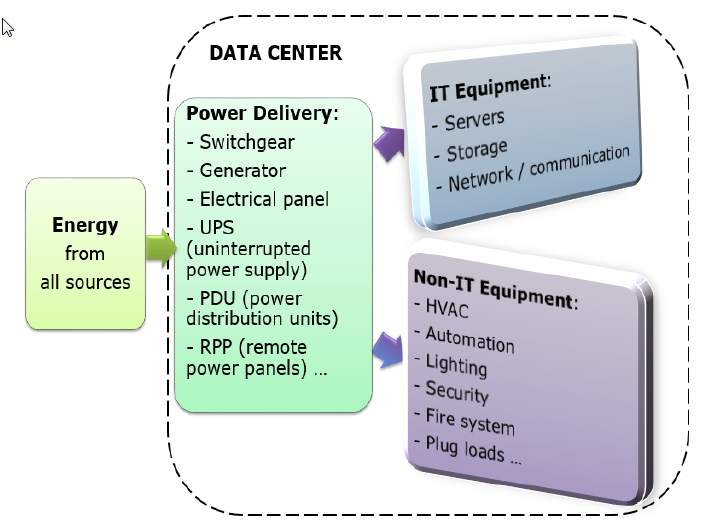
\includegraphics[scale=0.35]{Data_center_energy}
\end{figure}

%Currently, In terms of energy consumption, the entire Information and Communication Technology (ICT) sector including Data Centres now generates up to 2\% of the global CO2 emissions, which is on a par with the aviation industry.

Data Centres consume forty times more energy than conventional office buildings~\citep{edsdoj.99f37e7899fb4fcaabdaa81e395626c420180101} and have the fastest growing carbon footprint across the whole ICT sector~\citep{edsbas.13818AC20170101}.

Figure~\ref{fig:DCenergyEU-US}, reproduced from \citet{edsbas.13818AC20170101} shows the rising energy consumption of Data Centres across the EU and the US over the last 15 years as the number of Data Centres have grown:

\begin{figure}[h]
  \caption{Energy Consumption of Data Centres in the EU and US from 2000 to currently.}
  \label{fig:DCenergyEU-US}
  \centering
    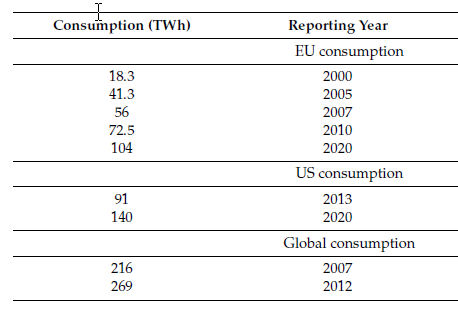
\includegraphics[scale=0.45]{Energy_consumption}
\end{figure}

With Data Centres consuming more energy, there is an obvious incentive, both from a cost and a green perspective, to reduce energy consumption per Data Centre. This can be done by making Data Centres more efficient for the energy they consume and the measurement that is used to measure energy efficiency is the \emph{Power Usage Efficiency} (PUE) score. This is described as

\begin{quotation} 
Power Usage Effectiveness = Total Facility Energy Usage/ IT Equipment Usage.
\end{quotation}

Lower PUE scores are better, and a PUE close to one indicates that the Data Centre is more efficient as it consumes less energy on non IT equipment such as cooling. 
In terms of the current trends of energy usage, research by \citet{edsbas.13818AC20170101} show that Data Centres in Northern Europe have a lower PUE score than those in southern Europe, which is expected given the geographical and climate difference. Also, the same authors find that the PUE scores in general have been decreasing year after year as demonstrated by the graphs in Figures \ref{fig:PUE-by-location} and \ref{fig:PUE-by-year}.

\begin{figure}[h]
  \caption{The average PUE across different locations.}
  \label{fig:PUE-by-location}
  \centering
    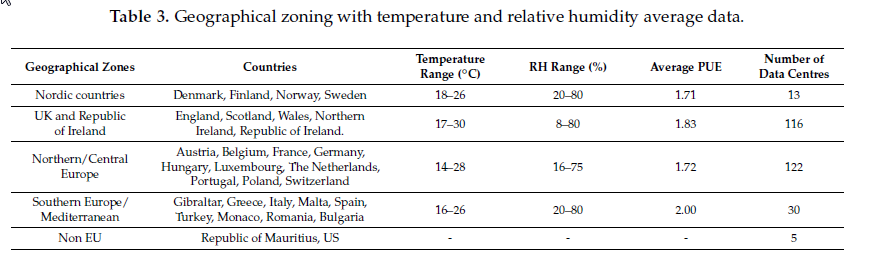
\includegraphics[scale=0.45]{geographical_zoning}
\end{figure}

\begin{figure}[h]
  \caption{The average PUE from 2000 to currently.}
  \label{fig:PUE-by-year}
  \centering
    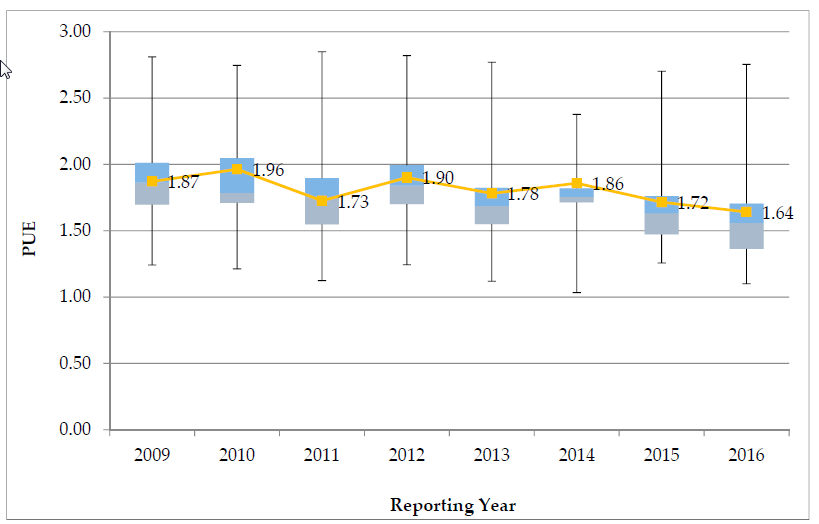
\includegraphics[scale=0.35]{Average_PUE_per_reporting_year}
\end{figure}
 
So the challenge, as outlined in the various literature below (section \ref{subsec:[Improving Data Centre Energy Efficiency]}), is how to make a Data Centre more energy efficient by maximizing the energy used for IT equipment and reducing the consumption of energy by non-IT equipment. 

\subsubsection{The WIT-TSSG Data Centre}
\label{subsubsec:[The WIT-TSSG Data Centre]}

The WIT-TSSG Data Centre is located on the Carriganore West Campus of the Waterford Institute of Technology (WIT) on the west side of Waterford city. From this location, the Data Centre supports over 50 concurrently active ICT research projects through provisioning of internet services, Cloud Computing resources, an AI cluster and project bespoke test beds \citep{TSSG}. 

In particular, the Data Centre supports TSSG projects, the Higher Education Authority, The Irish Centre for High End Computing(ICHEC), hosting its super computer Kay, Arclabs and other 3rd party commercial arrangements.

In terms of its energy usage, the Data Centre has an IT power load of 300kW, with cabinets engineered to house 30kW of IT equipment. 1+1 300kW UPSs and an 800kW Generator provide the backup power \citep{TSSG}.

With regards to physical hardware, the Data Centre supports over 160 physical servers, providing more than 1,000 cpu cores for processing and 400 virtual servers for cloud computing.  In addition, there is over half a PB (that is 512 TB) of Data Storage, and ~3,000 network port \citep{TSSG}. 

Figure~\ref{fig:TSSGdataCentreDesign}, provided from \citet{TSSG} demonstrates the design and infrastructure of the Data Centre building.  

\begin{figure}[h]
  \caption{The design of the WIT-TSSG Data Centre.}
  \label{fig:TSSGdataCentreDesign}
  \centering
    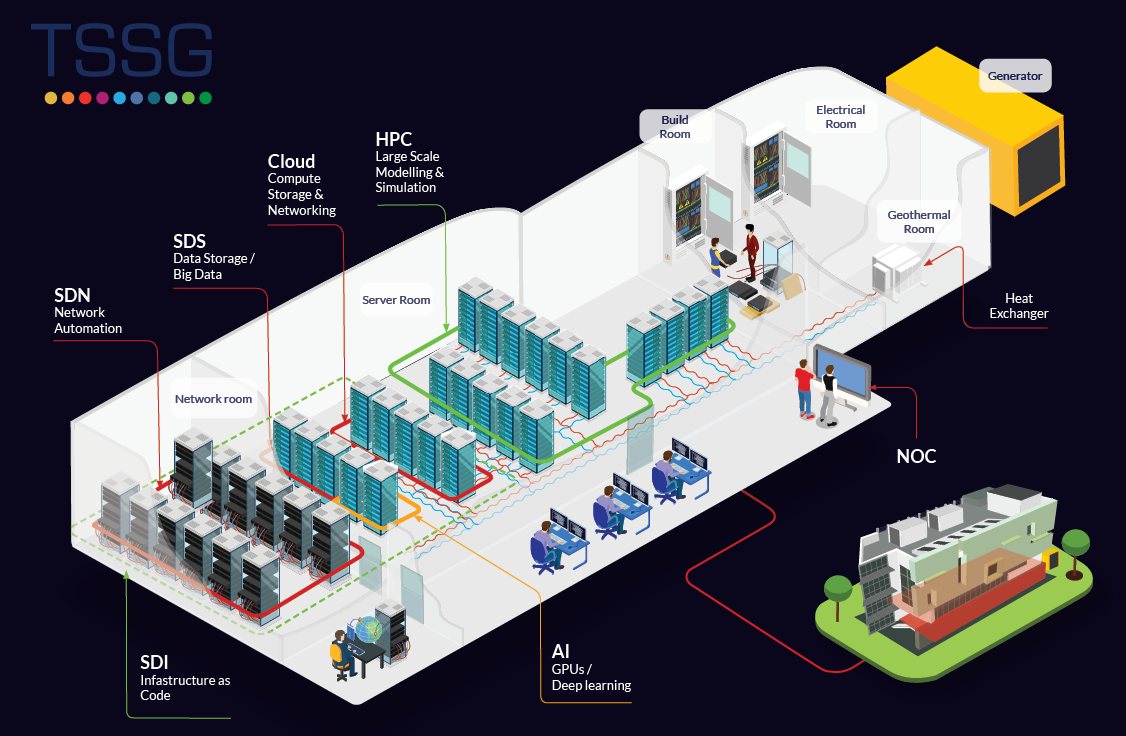
\includegraphics[scale=0.35]{TSSG_Diagram}
\end{figure}

From this diagram we see that there are 26 Cabinets and these use varying degrees of KW per cabinet to house over 160 servers. In addition, the Data Centre is designed so that there are separate rooms for servers, networking equipment, UPS and batteries with the generator and cooling equipment outside. This is to optimise the best cooling option for each room, resulting in the server room not having any hot or cold aisles. Instead, all heat and cooling is contained inside the 26 cabinets \citep{TSSG}.

In terms of a cooling system, the Data Centre uses a water based cooling system which uses less energy than an air cooled system. For monitoring and visualisation, the Data Centre uses Nagios and the ELK software stack \citep{ELK} with the output from that monitoring system is discussed further in section \ref{subsec:[Data Available]} and \ref{subsec:[Exploratory Data Analysis]} (Data Available and Exploratory Data Analysis). 

Also, as part of this research, Michael Kugel and John Ronan, who are Data Administrators at the Data Centre were interviewed to garner further information on the Data Centre. They were able to identify specific features that might warrant investigation and outline current projects to upgrade the Data Centre while they also outlined any anomalies I might expect to see in the monitoring data.  

In addition to this, when conducting the correlation analysis as outlined in section \ref{subsubsec:[Analyse Correlations]}, it became clear that further understanding was needed of the metrics involved and how energy consumption might be measured in a Data Centre. \cite{edseee.792155120170101} provide a comprehensive set of metrics and key performance indicators that are used in Data Centres that can be used to add context to the analysis of the WIT-TSSG Data Centre. 


\subsection{Improving Data Centre Energy Efficiency}
\label{subsec:[Improving Data Centre Energy Efficiency]}

From the Research Problem Statement (section \ref{subsec:[Research Problem Statement]}), the benefits for improving Data Centre energy efficiency is twofold: reducing the carbon footprint of the Data Centre, and reducing the cost of maintaining the Data Centre and these benefits should be mutually inclusive. Therefore, with such a desired outcome at stake, it is not surprising that a large amount of literature devotes itself to efforts in improving energy efficiency in Data Centres.

As outlined from the previous section (\ref{subsec:[Data Centre Infrastructure and the WIT-TSSG Data Centre]}), Data Centres are recent innovations, so to a degree, the literature is still catching up with the newest technologies and best practices. However, it is important to outline the earlier literature to understand why modern Data Centres, such as the WIT-TSSG Data Centre would have the ability to capture and store sensory data from its general operations. The following research summarises the need for such a sensor system and the immediate benefits this can bring to the energy efficiency of a Data Centre.   

To begin, a 2008 study by \citet{edsbas.A50BA51A20120101} states that implementing a sensor system to capture data can reduce energy demand by as much as 80\% through aggressive pursuit of energy efficiency measures specifically focussed around servers, while in 2012, the literature from this time also calls for the implementation of wireless sensors to begin capturing data. 

Here, \citet{edssch.qt9c84f49g20130101} argues that capturing this data via wireless sensors and then using integrated software to manage and integrate this into management systems can allow for greater efficiencies in a Data Centres cooling system and power usage, while \citet{edsjsr.4134817120120101} explain that a lack of visibility into a Data Centres operating conditions is an underlying reason for low-energy utilization. 

In this study, the authors argue for the introduction of sensor networks that combined with modelling, could provide insights into the distribution of energy and resolve the tension between cooling and performance.    

While these outlined the immediate and obvious benefits of integrating more reliable data into management systems and decisions, which by and large has been implemented, more recent literature investigates where more marginal gains can be found.  

\citet{edsdoj.47fdd5c4e23a43e3aa37ddd2fb75d82b20160101} looks to the performance of network capabilities and in particular, this research develops simulation models to predict the performance of networks based on the traffic through networks and concludes that the network performance models only lead to minor prediction accuracy degradation but the same models can accelerate the performance analysis by a much larger factor.  

\citet{edsarx.1402.080420140101} uses sensor data and a Map-Reduce computation in Hadoop to analyse server usage to maximise the efficiency of CPU power being used by each server in a Data Centre, thereby introducing some advanced data analysis of a specifically gathered sensor data. 

\citet{edsbas.DFD37F4F20160101} moved the argument on from creating sensor networks to developing a monitoring service for energy efficiency and sustainable management in Data Centres. The approach the authors use is to collect the monitoring data, analyse the data captured and then execute based on the outcome of the analysis. This is further developed today in Data Centres where centres use the TICK or ELK (section \ref{subsubsec:[The WIT-TSSG Data Centre]}).  

Another approach used to improve Data Centre energy efficiency in the literature is advanced by \citet{edsdoj.99f37e7899fb4fcaabdaa81e395626c420180101} who introduce a whole new set of metrics to review the efficiency of Data Centres. They argue that while the old metrics are valuable, some key metrics concerning \emph{risk} are overlooked. They advance a new Data Centre multidimensional scorecard which gives better visualisation to identify areas of improvement. 

More advanced initiatives are based around the optimisation of physical resources within a Data Centre. \citet{10234066620151001} propose a multi-tier architecture-orientated virtualised application performance model to allocate computing resources to each machine based on SLA (service level agreement) restrictions. The authors develop a heuristic mixed optimisation algorithm to achieve this.

Finally, \citet{VASUDEVAN201794} seek to reduce the operational costs of Data Centres and maximise energy efficiency by analysing log data to profile applications using the Data Centre. In addition, the authors profile the virtual and physical machines in the Data Centre, and using a penalty-based matching algorithm match different applications with the most compatible machines (virtual and physical) so that CPU usage is more efficient. 

The literature outlined here demonstrates the changing focus of how best to increase the energy efficiency of data centres. From early calls, just ten years ago, to implement sensor systems to that would lead to improved management systems and easily identified gains, to more recent and more advanced techniques looking to use algorithms to increase optimisation of the resources in a Data Centre. In all cases highlighted, the importance of capturing, understanding and using data to integrate new information into management systems and operations is stressed. However, in these instances, the approaches identify explicit data they want to capture and analyse, whether this is log data on CPU utilization or specific monitoring data. In general, few Data Mining approaches are used, in the sense of using implicit data to uncover hidden insights. The research questions in section \ref{subsec:[Research Questions]} focuses on this concept.  


\subsection{Data Mining Techniques (for improving energy efficiency in buildings)}  
\label{subsec:[Data Mining Techniques]}
Data Mining is the process of uncovering hidden patterns from large sets of data, where the data is analysed to extract information which can be transformed into valuable knowledge for the future. Such techniques include statistical and machine learning techniques which take the form of regression analysis, classification, cluster analysis and more advanced techniques such as neural networks. These techniques analyse the relationship between variables to uncover such hidden patterns and trends.  

While there is limited literature or existing research on using Data Mining techniques to improve the energy efficiency of Data Centres, there is comprehensive research on using Data Mining approaches to assess the energy efficiency of buildings in general, or of various systems within buildings. Because a Data Centre is a building in its own right, it is important to review such Data Mining techniques in the building management literature and assess if the research can be applied to Data Centres.   

In general, the literature can be divided into two sections, where basic Data Mining techniques are used, as described above, and when more complex algorithms are used to gain insights. First, I explore the literature on the basic Data Mining approaches.
 
\citet{XUE2017926} look at district heating substations in Northern China, and from operational data collected from the substations use clustering techniques to identify seasonal and daily operating patterns, and association rules mining to identify faults, malfunctions and inefficient operations strategies. 

\citet{JEFFREYKUO2018120} uses regression and classification techniques on different factors in analysing the energy consumption characteristics of Taiwan's convenience stores. The data is collected from a survey of convenience stores owners before the Data Mining techniques look at intercorrelation between energy consumption and other factors such as geography, climate and store design. 

Using operational data from the construction of an education building in Hong Kong University, \citet{FAN2018296} use decision trees, motif discovery and gradual pattern mining to uncover novel and valuable insights for the management of energy consumption for the building.

Also, using monitoring data from building automation systems, \citet{FAN2018296} explore how unsupervised Data Mining techniques such as clustering, association rule mining, motif discovery and unsupervised anomaly detection can be used to gain insights into energy efficiencies within buildings. 

In a similar study by \citet{ZHOU201873}, the authors use data supplied from heat supply companies in Singapore and look at the correlation between energy consumption and building physics, the heating system and room position, and use the information gain ratio algorithm and decision tree classifiers to analyse energy consumption and other related factors. 

\citet{AHMAD2018460} use Gaussian process regression, multiple linear regression, tree bagger, bagged tree, boosted tree and neural networks to identify abnormal behaviour and predict the future heating and cooling demands in building environments. 

These approaches will be reviewed when finalising a predictive model for energy consumption in section \ref{subsubsec:[Finalise Predictive Model]}. However, in addition to those highlighted, further literature has been sourced that specifically concentrated on analysing energy consumption in a Data Centre. \citep{Makris2017} collects data from the Data Centre processor, access memory and the network interface controller and analyses these features using linear regression to predict energy consumption at a system-level.

A precursor to the regression analysis is correlation analysis as outlined in section \ref{subsubsec:[Analyse Correlations]}, and it was important to understand the value this can bring to a data mining approach. \citep{13375977120180401} use multivariate correlation and data mining clustering techniques for detecting distributed denial of service attacks in cloud computing. Specifically, the authors investigate the correlation among selected and ranked variables. Such an approach is used in this project to identify predictive features of energy consumption and pinpoint potential inefficient energy consumption.    

However, some research also uses more advanced algorithms to gain hidden insights from the data captured. 

\citet{13090171620180801} use log data and the self-organising maps algorithm to create a decision support application for anomaly detection in IT systems. They highlight that this algorithm is used in anomaly detection in fraud cases and security attacks, but most importantly they highlight, when using the log data from systems, the self-organising maps algorithm allows for early detection of failures in critical systems in real-time. 

The Random Forrest Algorithm is used by \citet{WANG2017251} to discover critical events for event driven optimisation in building air-conditioned systems. With data collected from the building automation system, the authors make a case for using Data Mining to gain efficiencies in air conditioned systems by moving away from a time based system, to a more event driven optimisation.  

The literature reviewed at this point highlights the wide and varied Data Mining approaches taken by various authors to gain hidden insights into energy efficiencies within buildings or building systems such as heating or cooling systems. 

This project will adapt these approaches to the monitoring data we have gathered from WIT-TSSG Data Centre to help answer our Research Questions (section \ref{subsec:[Research Questions]}).   

\subsection{Summary}  
\label{subsec:[Summary]}
While the literature review is ongoing, the research questions above (section \ref{subsec:[Research Questions]}) clearly set out the goal of maximising energy efficiency within a Data Centre and the ongoing literature review sets out the framework for building the foundations for this research. Firstly, it defines what a Data Centre is and the trends in energy consumption by Data Centres (section \ref{subsubsec:[What is a Data Centre and How Much Energy do they Use?]}) before introducing the WIT-TSSG Data centre in Waterford (section \ref{subsubsec:[The WIT-TSSG Data Centre]}). From these foundations, the literature review focussed on various computational and systematic improvements that could lead to greater energy efficiency within a Data Centre (section \ref{subsec:[Improving Data Centre Energy Efficiency]}). The importance of wireless sensory data is a common starting point for most authors who focus on efficiency improvements to be made by concentrating on hardware improvements (network, server or cooling systems). Most of these approaches use data which is specifically captured at a system level to assist the goal of increased energy efficiency.

This is where I believe there is a research gap. Data Centres are entities in their own right and store vast amounts of operational and monitoring data. This has been harvested by a monitoring system and could be useful to analyse, using Data Mining techniques, to find hidden insights around energy efficiency. 

Based on this, the final section of the literary review looked at where Data Mining techniques are used for similar applications (section \ref{subsec:[Data Mining Techniques]}) such as the energy efficiency of different building types, or heating or cooling systems within a building. Various Data Mining techniques are explored in the literature and are assessed to see if such approaches can be adapted for use in a Data Centre.   

The nature of this research dictates that the literature review will never be a defined and finished section. Since the proposal stage, further research has investigated the usefulness of correlation analysis, defined metrics for Data Centres, and purposefully, a paper outlining a proposal for predicting energy consumption in a Data Centre. Furthermore, if Research Question 3 is pursued, further research will be required to appreciate the technical aspects of the Chiller operations of the Data Centre. 

\section{Working Theory}
\label{sec:[Working Theory]}
From the literature reviewed up to this point (section \ref{sec:[Ongoing Literary Review]}), there was a gap identified where data mining techniques could be used on the monitoring data compiled within a Data Centre to unlock hidden sources of information that could lead to greater energy efficiency in operating the Data Centre. The research questions (section \ref{subsec:[Research Questions]}), ask if these efficiencies could brought about either by being able to predict when energy demand peaks in order to better utilise the supply of energy that the Data Centre is using or also identify anomalies in the Data Centre where energy is not being used efficiently. 

Whereas the majority of literature analyses the hardware components of a Data Centre to improve efficiency (section \ref{subsec:[Improving Data Centre Energy Efficiency]}), this research proposes to concentrate on the energy demand of a Data Centre. At any given time, a Data Centre will have a certain load to process, and will utilise it's available resources to process the load. To maximise efficiency therefore, a Data Centre would need to be able to best match the energy demand with the supply at its disposal. The real gains in efficiency therefore, is to be able to anticipate the demand to best utilise the resources at its disposal. In technical terms, this would mean moving loads between racks within a Data Centre or reducing the demand for the cooling system at certain times. 

Therefore, to increase the efficiency of a Data Centre by concentrating on energy demand, we need to anticipate the demand of energy usage. This proposal seeks to create such a predictive model using the Data Mining techniques outlined in the literature review (section \ref{subsec:[Data Mining Techniques]}) and the monitoring data collected from within the Data Centre (section \ref{subsec:[Data Available]}). This model is currently being constructed following detailed correlation analysis as outlined in section \ref{subsubsec:[Analyse Correlations]}

If a good predictive model of energy demand can be built, this will be the missing piece of the jigsaw in helping the Data Centre become more efficient by analysing its own monitoring data to anticipate a surge in energy demand. This in turn will allow the Data Centre to utilise its supply of energy, making it more energy efficient and aligning with our aim of reducing the cost of running the Data Centre (section \ref{subsec:[Aims and Objective]})

In addition to this stream of work, we can use correlation analysis and further investigations to potentially highlight inefficiencies in the management of the chiller operations. However, as outlined in the research questions section (\ref{subsec:[Research Questions]}), this is contingent on the participation of key personnel, and their technical knowledge of the area, to assist in that effort. As stated there are significant rewards to bringing this work to fruition, but also high risk in that there are no guarantees that the resources required will be available in the remaining lifespan of this project. Time spent pursuing this stream of work will require careful judgement and the situation will have to managed accordingly.     

In conclusion, this project is treating a Data Centre as an entity in its own right. Instead of merely being an end point in a cloud computing infrastructure for many applications or physical machines, it is utilising the data created by the Data Centre itself. By doing this, a predictive model is being built to anticipate the demand of energy needed, thereby transforming the Data Centre from being an intricate part a cloud computing framework to a more Edge orientated framework in its own right.     

\section{Research Methods}
\label{sec:[Research Methods]}
This section builds on the Working Theory and firstly introduces the data available to this study before delving further into how a predictive model will be constructed using the data available.

\subsection{Data Available}
\label{subsec:[Data Available]}
As outlined in section \ref{subsubsec:[The WIT-TSSG Data Centre]}, the Data Centre examined is the WIT-TSSG (Telecommunications, Software and Systems Group) Data Centre in the Carriganore West Campus, part of the Waterford Institute of Technology (WIT). The Data Centre was completed in January 2010 in order to support its network-based research projects in the area of telecommunications networking and cloud computing. The Data Centre was designed with high-density, power efficiency and separation of services as its primary goals. It has a total IT power load of 300Kw with some cabinets engineered to house 30kw of IT equipment.

Similar to most modern Data Centres, sensors and the use of network devices are used to monitor and capture data on how the Data Centre is operating. As outlined in the schema model shown in Figure \ref{fig:TSSGdataschema} below, there is substantive qualitative data captured that can be used for the empirical investigations to create a predictive model.  

\begin{figure}[h]
  \caption{The schema of the WIT-TSSG Data Centre.}
  \label{fig:TSSGdataschema}
  \centering
    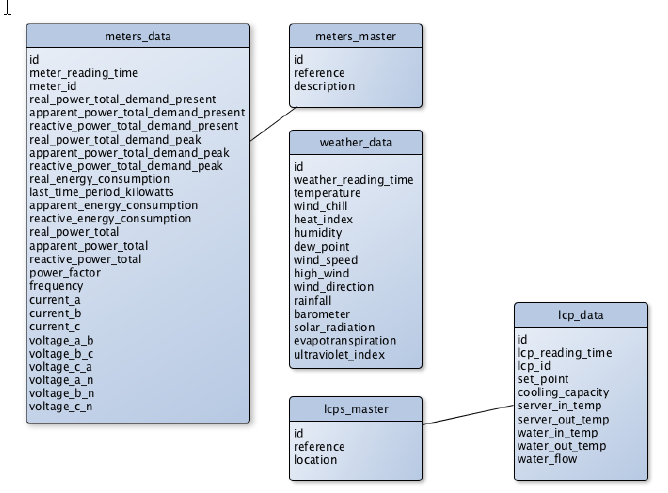
\includegraphics[scale=0.45]{TSSG_Data_Schema}
\end{figure}

As we see from the schema, the data captures a multitude of metered energy usage variables, different weather data, and temperature and water usage data. A full detailed definition of the key metrics is provided in the appendices - section \ref{sec:[Definition of key Variables]}. The data outlined here is available from 2014 right up to present, captured at 5 minute intervals, making this a time series data set. In the next section, the data is explored at an initial level to find any seasonal trends or predictive variables. 
 
\subsection{Exploratory Data Analysis}
\label{subsec:[Exploratory Data Analysis]}
The data analysed for this project is a static 'data dump'. Additional data, when available, can be added to the study if required. The data was accessed by connecting remotely into the Data Centre via PuTTY and querying the data via MySQL (See Appendices - section \ref{sec:[MySQL Queries]}). From here, the CSV output from the SQL queries was SFTP'd to my local machine and exported into Microsoft Excel where some preliminary data analysis was carried out. 

The schema introduced in Figure \ref{fig:TSSGdataschema} outlines the vast scale of variables available and as such data is gathered in 5 minute intervals over four years, the amount of data accumulated is vast and can be challenging to work with. While Python is used for developing the Data Mining Techniques (see section \ref{subsec:[Data Mining Techniques]})  line charts are ideal to illustrate, at an exploratory level, what the time series data can show and the following charts are snippets from the data to demonstrate the range of data available.

\begin{figure}[h]
  \caption{Energy consumption (in kW usage per 5 minute intervals) of one cabinet in the Data Centre over the entire year of 2017.}
  \label{fig:Annualenergyfigure}
  \centering
    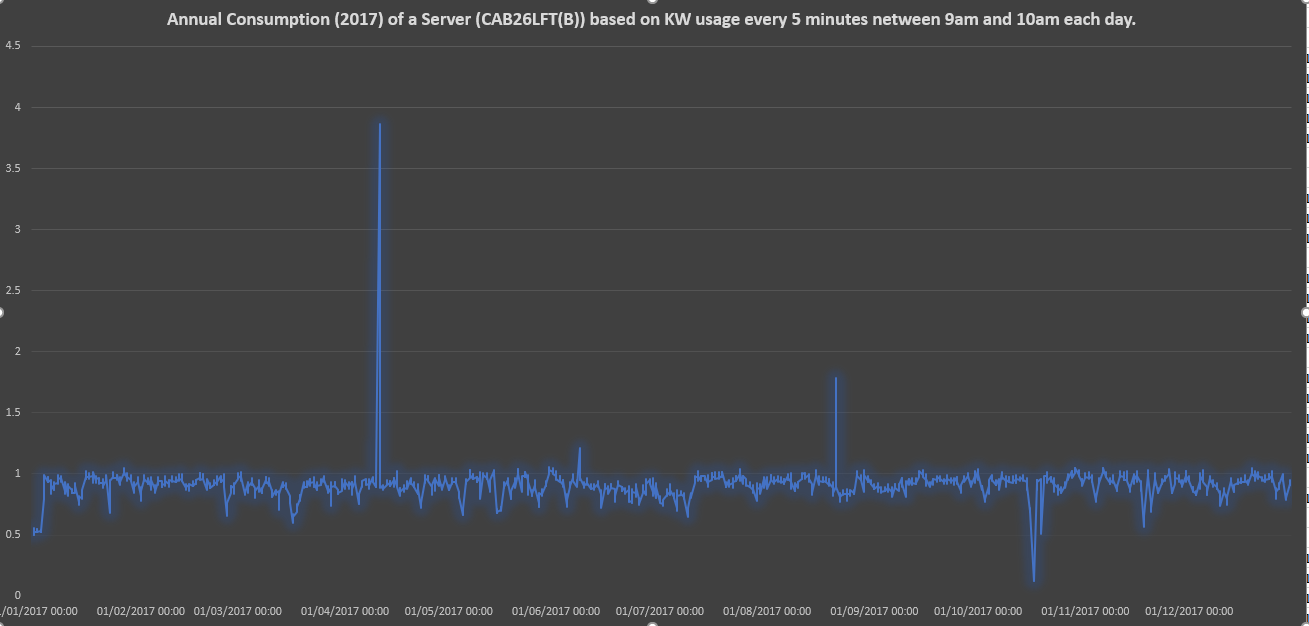
\includegraphics[scale=0.30]{Annual_energy_consumption}
\end{figure}

Figure \ref{fig:Annualenergyfigure}, generated using Listing~\ref{list:[Annual Energy Consumption]}, illustrates the energy consumption of one particular server cabinet within the Data Centre (Cabinet 26A) over the course of 2017. The daily readings are taken from between 9am and 10am each day and while the chart may initially suggest that the energy usage has been relatively consistent, there are significant spikes in energy consumption in April and August, with some considerable drops in demand too. The Research Techniques section (\ref{subsec:[Research Techniques]}) will outline how this study investigates if these spikes can be predicted so that another cabinet could share some of the load to reduce energy consumption within the Data Centre.

However, while Figure \ref{fig:Annualenergyfigure} was a snapshot of energy usage over a year, the data can also be presented for a particular day. 

\begin{figure}[h]
  \caption{Energy consumption (in kW usage per 5 minute intervals) of three different server cabinets in the Data Centre over the course of one day (2017-09-13).}
  \label{fig:Dailyenergyfigure}
  \centering
    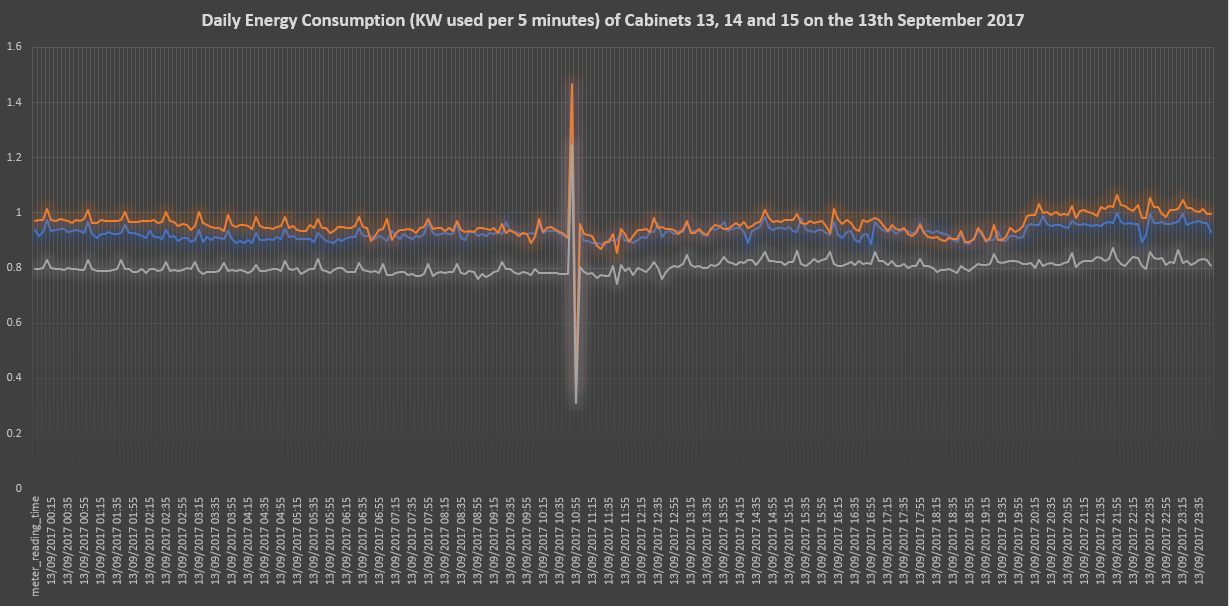
\includegraphics[scale=0.35]{Daily_energy_consumption_of_cab131415}
\end{figure}
   
Figure \ref{fig:Dailyenergyfigure} reports significant spikes in energy consumption in two of the cabinets around 11am. Again, this is another example of how Data Mining techniques might be applied to assist in being able to predict when such spikes occur. 

While certain spikes in energy consumption might be suitable for further investigation, the preliminary data analysis should be able to detect some seasonal behaviour. Figure \ref{fig:cabvchillerfigure} demonstrates this. While the energy usage for the server cabinet (cabinet 26b) is relatively stable throughout the year, the energy consumption for the chillers shows a clear increase throughout the warmer summer months. Interestingly however, while each chiller works on alternate weeks, there are unexplained spikes for chiller B throughout the second half of the year that are not replicated when chiller A is running. 

\begin{figure}[h]
  \caption{Energy consumption (in kW usage per 5 minute intervals) of both Chillers and one server cabinet in the Data Centre over the course of 2017}
  \label{fig:cabvchillerfigure}
  \centering
    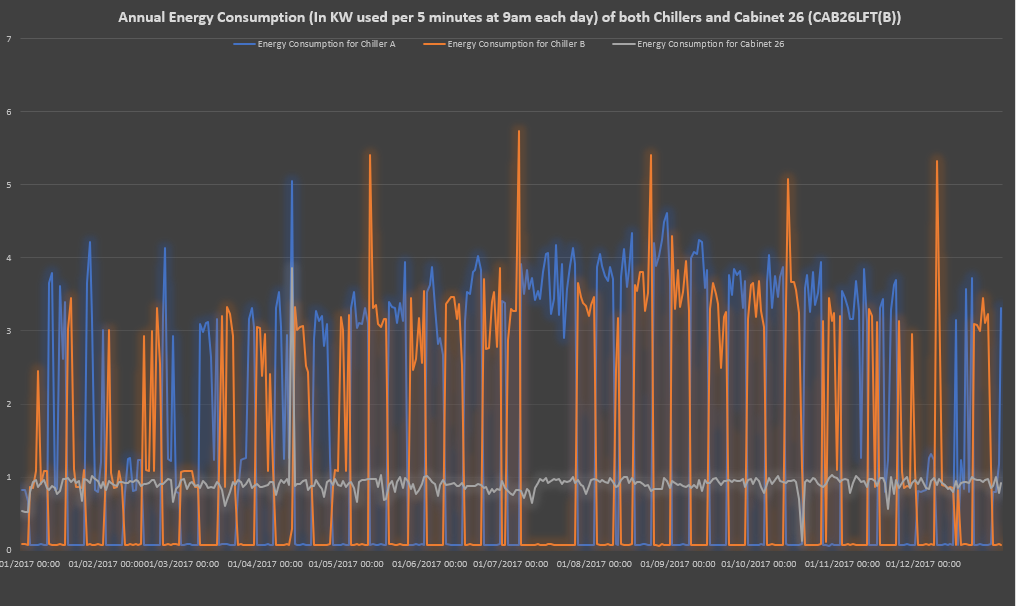
\includegraphics[scale=0.45]{Energy_consumption_of_cab26_and_chillers}
\end{figure} 

It is from presenting this information to Michael Kugel and John Ronan who work in the Data Centre, where the impetus came to specifically concentrate on the inefficiency of the chiller system. It was their 'hunch' that such inefficiencies existed, and it was these discussions that spawned the third research question (in section \ref{subsec:[Research Questions]}) and possible further investigation as outlined in sectio/ \ref{subsubsec:[Further Analysis of the Chiller System]}.   

Other interesting preliminary analysis of the data centred around water consumption at the Data Centre (Figure \ref{fig:annualwaterfigure} ) and the energy usage of the generator during a severe weather event, in this case being Storm Ophelia on October 2017 (Figure \ref{fig:opheliafigure} ). 

\begin{figure}[h]
  \caption{Annual water flow (in litres per 5 minute intervals) to LCP 1 measured at 9am every day during 2017}
  \label{fig:annualwaterfigure}
  \centering
    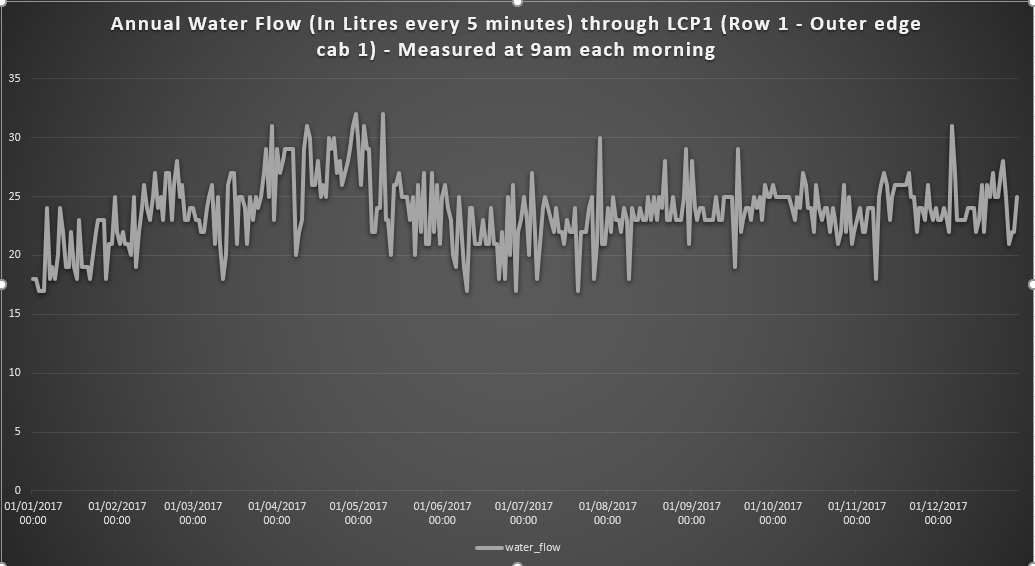
\includegraphics[scale=0.45]{Annual_Water_Flow}
\end{figure} 

\begin{figure}[h]
  \caption{Energy consumption (in kW usage per 5 minute intervals) of the Generator before, during and after Storm Ophelia in October 15th 2017}
  \label{fig:opheliafigure}
  \centering
    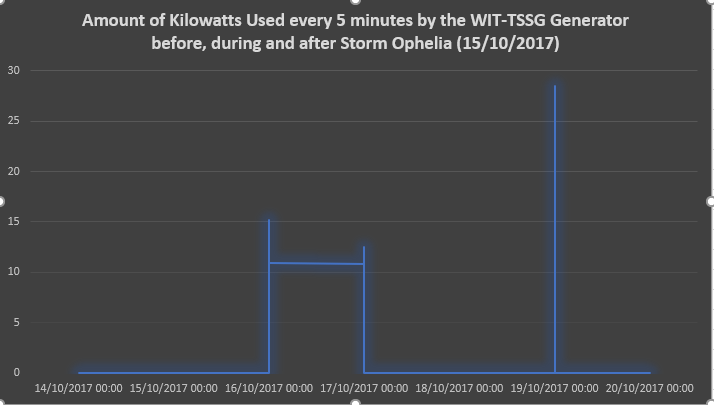
\includegraphics[scale=0.50]{Ophelia_generator}
\end{figure} 

All these charts are provided to simply demonstrate the range of data available. The next section discusses how this data was screened to build a predictive model and the challenges that arise from this.  

\subsection{Research Techniques}
\label{subsec:[Research Techniques]}
An advantage for this research is that the data required is already available for analysis and the previous sections (\ref{subsec:[Data Available]} and \ref{subsec:[Exploratory Data Analysis]}) introduced the variables and did some exploratory data analysis. This section progresses further, and outlines how the data will be screened to build a predictive model as outlined in the Working Theory. 

Figure's \ref{fig:Annualenergyfigure}, \ref{fig:Dailyenergyfigure}, \ref{fig:cabvchillerfigure}, \ref{fig:annualwaterfigure} and \ref{fig:opheliafigure} demonstrate that the data available here is time series data. With data going back to 2014, this allowed for investigations into the energy usage per cabinet, per rack or even at a system level, whether that is the energy consumed by the network configuration, the server demand or other computational needs. 

This study, using Data from 2017 specifically, then used correlation analysis to discover predictive variables of when energy demand peaks and also to highlight any anomalies in the performance of the chiller system. The Exploratory Data Analysis section (\ref{subsec:[Exploratory Data Analysis]}) even highlighted instances of when demand actually peaks and predicting this would be helpful as it will allow the system administrators to manage the supply of energy better at these peak times, thereby increasing the efficiency of the data centre. The Exploratory Data Analysis section (\ref{subsec:[Exploratory Data Analysis]}) also illustrated seasonal effects where energy demand will increase in the summer months of the year as the warm weather precipitates the need for greater cooling within a Data Centre. However, the approach here will be to analyse these factors at a deeper level to build a more developed predictive model that unlocks hidden insights not yet discovered.

To carry out the correlation analysis the data was imported into Python for detailed Data Mining exploration to generate the correlations. The output from this is outlined in section \ref{subsubsec:[Analyse Correlations]}. The next step was to review the literature reviewed above (section \ref{subsec:[Data Mining Techniques]}) and the various Data Mining techniques that have been used to increase energy efficiency of different building and heating systems. Some of these are utilised here to identify predictive variables and build a predictive model (section \ref{subsubsec:[Construct Predictive Model]}).

From here, and the next steps in the project, regression analysis will look at the relationship between variables and predict a quantitative output, so potentially this could predict energy consumption by looking at different servers combined with weather information or the supply of water to the chiller systems. The objective would be to find ways of deriving suitable features to improve the model predictions. Clustering techniques could be used to look at the relationships between these predictors and derive some  intuition regarding correlations between different events and problems with the chillers. These are just some examples that will be explored but ultimately at this stage of a project, the exact method is not known yet. There will be a degree of trial and error in finding the exact method and the most suitable data. 

However, a predictive model is only useful if it's predictable and reliable, meaning it should be accurate and precise. In attempting to develop such a model it will be important to focus on goodness of fit measures like bias and variance. This will be a key factor in the project also.

Finally, as outlined in section \ref{subsec:[Data Available]}, it is important to note that the data presented here is a static 'data dump'. This allows for the development of predictive models on the static data only. However, an advantage of having nearly five years of static data is that it allows for the model to be tested on different subsections of the data to test its validity and reliability.  Therefore data from 2017 has been used in the analysis so far, meaning data from other years can be used to test any predictive model. While this is useful and would solve for our research questions (section \ref{subsec:[Research Questions]}) concerning increasing energy efficiency within a Data Centre, a more ideal model would be based on live streaming data. This would allow us to solve for problems outlined in real-time and develop models that will assist in anomaly detection or highlight when system failures might occur in real time and assist in avoiding such failures. 

\section{Progress Report}
\label{sec:[Progress Report]}

\subsection{Original Project Plan}
\label{subsec:[Original Project Plan]}
The plan of work, as originally proposed, for this project is outlined in the Gantt chart in Figure \ref{fig:projectplan} below. The  tasks had added contingency to avoid a chaotic and disordered critical path and align with the key milestone dates for Thesis submission as outlined by WIT authorities. 

\begin{figure}[h]
  \caption{Project Plan for 2018-2019.}
  \label{fig:projectplan}
  \centering
    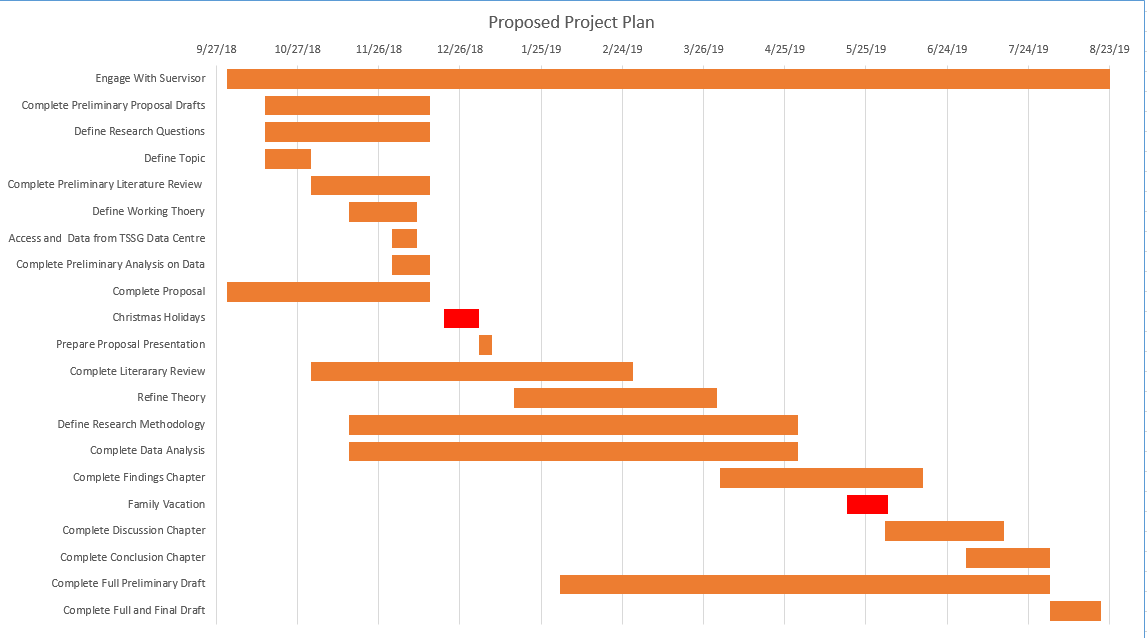
\includegraphics[scale=0.45]{Gannt_Chart_schedule_of_work}
\end{figure}

\subsection{Progress Since Proposal}
\label{subsec:[Progress Since Proposal]}

The Aims and Motivations (section \ref{subsec:[Aims and Objective]}), Research Questions (section \ref{subsec:[Research Questions]}), Literature Review (section \ref{sec:[Ongoing Literary Review]}), Working Theory (section \ref{sec:[Working Theory]}) and Research Techniques (section \ref{subsec:[Research Techniques]}) have all been impacted by how the project has proceeded since the proposal stage. That specific progress is detailed here.  

\subsubsection{Import Data From Data Centre}
\label{subsubsec:[Import Data From Data Centre]}

The first step was to retrieve the monitoring data for 2017 that is stored on the server of the Data Centre. Similar to the section \ref{subsec:[Exploratory Data Analysis]}, data was exported from the Data Centre by logging on remotely via PuTTY and directly querying the data, using MySQL (See Appendices - section \ref{sec:[MySQL Queries]}) and SFTP'ing the query results, as csv files, to my own local machine. 

Caption \ref{fig:TSSGdataschema} as previously outlined, visualises what data is available in the Data Centre. Specifically, data from 2017 was used as an initial testing sandbox for the data analysis. This allows the data for other years to be used to validate any findings. As the time series data is gathered in 5 minute intervals, this equates to 175,200 entries for the entire year. 

In addition, specific monitoring data containing energy information from all 83 meter locations, \gls{LCP} information for all 15 \gls{LCP} locations and a11 weather variables were exported from the Data Centre. In total, for just 2017, that equated to over 210 million unique data entries, stored on three different csv files. 

\subsubsection{Understanding the Data}
\label{subsubsec:[Understanding the Data]}

With such a vast array of information available, as earlier demonstrated in section \ref{subsec:[Exploratory Data Analysis]}, the next stage was to streamline the amount of variables to be considered. After consultation, the following were chosen.  

\begin{figure}[h]
  \caption{Schema of Data and Variables chosen for detailed Data Analysis}
  \label{fig:finalvariables}
  \centering
    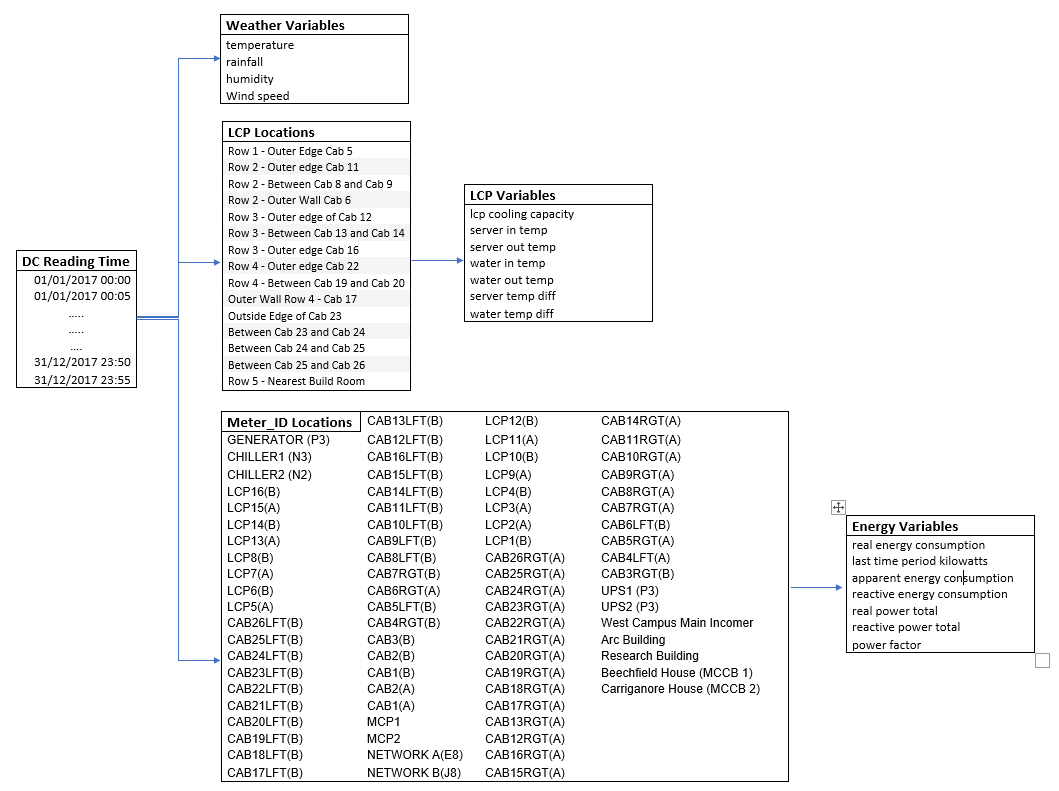
\includegraphics[scale=0.40]{finalvariables}
\end{figure} 

%While full definitions of the key variables are defined in the appendices - section \ref{sec:[Definition of key Variables]}, the following diagram describes and outlines the relationship between Real Energy Consumption, Reactive Energy Consumption, Apparent Energy Consumption and Power Factor. 
While full definitions of the key variables are defined in the appendices - section \ref{sec:[Definition of key Variables]}, the following diagram describes and outlines the relationship between \gls{Real}, \gls{Reactive}, \gls{Apparent} and \gls{Power}. 

\begin{figure}[h]
  \caption{The Latte Definition of Different Energy Metrics}
  \label{fig:coffeeenergyanaliogy}
  \centering
    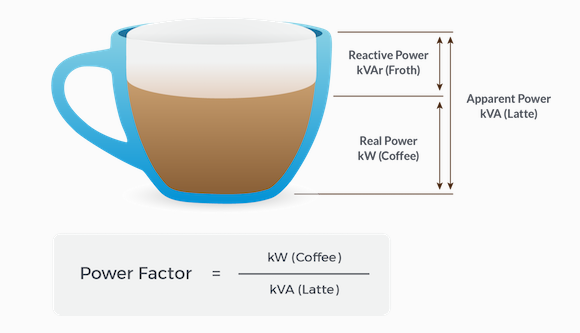
\includegraphics[scale=0.50]{power_explanation}
\end{figure} 

\subsubsection{Manipulate Data in Python}
\label{subsubsec:[Manipulate Data in Python]}

With the data now gathered from the Data Centre, and the key variables identified, the next stage was to use Python to create correlations between the variables to identify some predictive features. The following steps were carried out in Python and the full code is viewable in section \ref{sec:[Python Code]} of the appendices.

\begin{enumerate}
\item Import csv's to Python.
\item Streamline data to only include selected variables. 
\item Use Pivot Tables to generate data based on the DC Reading time for every location and associated variable. 
\item Merge all energy, \gls{LCP} and weather information together to create a master table of all data based on the 5 minute interval values (merged on DC Reading Time).
\item Generate correlations based on the created time series for all 690 variables.
\item This created nearly 240,000 correlations. From this Python was Instructed to export the top 45,000 correlations for further analysis
\end{enumerate} 

Ideally, during this process efforts would be made to reduce the dimensionality of the data so that further Python based analysis could take place such as heat maps. Unfortunately, any efforts with such an array of data was not possible due to computational limitations and while further attempts to do this later in the process may be pursued, at this time it was deemed that it was more important to explore the all variables identified.

\subsubsection{Analyse Correlations}
\label{subsubsec:[Analyse Correlations]}

The process to identify 'interesting' or 'useful' correlations was manual. Having received the top 45,000 correlations from Python, which had a correlation higher than +/- 0.93, this manual piece was done by importing the correlations to Microsoft Excel and using filters to trial and error different combinations. 

Some correlations between variables were easily explained, such as the relationship between different energy variables but the following are the initial findings:    

\begin{itemize}
\item There is a strong correlation between Humidity (but not temperature) and Real Energy Consumption, Apparent Energy Consumption and Reactive Energy Consumption.
\item There is a high correlation between Apparent Energy Consumption and Real Energy Consumption. This indicates that there is a relatively stable amount of reactive power generated at each meter.
\item There is a high amount of correlation between Real power total and Last time kw.
\item In terms of analysing the different performances of the chillers, out of 2103 correlations, 2089 are identical for both Chiller 1 and Chiller 2. The main difference centres around some correlations for Chiller 2 and the \gls{LCP} and server temp differences between cabinets 23/24 and 25/26.
\item Similarly, the water in temp and server in temp of the locations (between cabinets 23/24, 24/25, and 25/26) is highly correlated with the water in temp and server in temp of some locations between rows 2,3 and 4.
\item In terms of cross-correlations between meter id’s and LCP locations, there is a high correlation between Real Energy Consumption of most meter id’s and 5 particular \gls{LCP} variables that is very consistent.
\end{itemize}  

Full details of the correlation analysis, including a definition of the key variables discussed are found in the Appendices - sections \ref{sec:[Definition of key Variables]} and \ref{sec:[Correlation Analysis Results]}

\subsubsection{Meet with Data Centre Administrators}
\label{subsubsec:[Meet with Data Centre Administrators]}

Various meetings with Data Centre Administrators Michael Kugel and John Ronan took place during this process. These ranged from tours of the Data Centre, to in-depth discussions around possible areas of investigation and also detailed discussions around preliminary findings. 

In particular, they highlighted the inefficiencies in the Chiller system. Specifically, they explained how the two chillers alternate weeks in operation and how chiller 2 uses considerably more energy when it kicks in for its rotation.

It's from these meetings, that the third research question around the energy inefficiency of the chiller system got initially prioritised. The Data Administrators have a cost incentive to correctly identify the issue at stake, so that the specific hardware component can be replaced in isolation. Because without precisely identifying the component at fault, the cost of repairing the system increases exponentially. 

Therefore, from the Data Administrator's perspective their stated priority is to investigate the issues around the chiller system more so than predicting energy demand. However, as explained in the research questions (section \ref{subsec:[Research Questions]}, to prioritise this stream of work will require hands-on participation from the Data Administrators through to the end of the project. This is because of their technical knowledge of the electrical and plumbing systems associated with the chiller system. They also have access to further data around the water pressure within the system that is not available to me currently. So for this stream of work to reach a successful conclusion, the Data Administrators need to become partners in the research, not just consultants. At this stage, without this being confirmed, the third research question is only under consideration at this time, with the situation being actively managed in the short term to balance the overall priorities of the project.  


\subsubsection{Construct Predictive Model}
\label{subsubsec:[Construct Predictive Model]}

As per the \ref{subsec:[Research Questions]}, there are two distinct aspects of this work. Predicting energy usage and anomaly detection. In terms of predicting energy usage, the outcome of the correlation analysis allows us to use the variables identified to build a predictive model. At this stage, the data appears to intimate that humidity is correlated to an increase in energy consumption. This could be used along with some other variables to build a function to predict energy consumption, thus essentially becoming a regression problem. 

From the correlation analysis, the main variables to build such a model would be humidity, The server temp diff Row 3 - Outer edge of Cab 12, water flow Between Cab 23 and Cab 24 and lcp cooling capacity Between Cab 23, Cab 24 and Cab 25

In terms of anomaly detection, in general, regression would be used to investigate if residuals have either structure or isolated large deviations, which would warrant further investigation. 

\subsection{Remaining Work To Do}
\label{subsec:[Remaining Work To Do]}
This section outlines what the remaining steps are and the time-line to complete these steps.

\subsubsection{Finalise Predictive Model}
\label{subsubsec:[Finalise Predictive Model]}

Having begun constructing the predictive model, it is important to refine this further taking on board feedback from Data Centre administrators and other experts. This will also include deeper analysis of the correlations to ensure no hidden predictive features are missed and to review the existing literature outlined in section \ref{subsec:[Data Mining Techniques]}. The data already available for 2017 in Python could be used to smoke test the predictive model using regression tools available from Pandas. This phase should be complete by mid May. 

\subsubsection{Test Predictive Model}
\label{subsubsec:[Test Predictive Model]}

Having refined the model using 2017 data, the next step would be to test the model on data from other years. To do this, the data would be queried, stored and imported to Python as outlined in sections \ref{subsec:[Exploratory Data Analysis]} and \ref{subsubsec:[Import Data From Data Centre]}. Any detailed regression analysis should be undertook in Python that should also include goodness of fit measures to test the validity of the model. This should be completed by the end of June.  

\subsubsection{Further Analysis of the Chiller System}
\label{subsubsec:[Further Analysis of the Chiller System]}

Should this stream of work continue, with the risks and rewards outlined in section \ref{subsubsec:[Meet with Data Centre Administrators]}, this will take the following course of action: 

\begin{enumerate}
\item Obtain the water pressure data from the Data Centre. 
\item Build this information into the correlations already produced. 
\item Identify specific points in time where energy consumption of chiller 2 spikes. 
\item Work with Data Administrators to understand the outcome of this data analysis. 
\item Use the Data Administrators knowledge to drive further analysis of key components.  
\end{enumerate} 

This work will need to be completed by July, and the end goal from this to identify specific components that are failing and causing malfunctions in the chiller system. 

\subsubsection{Analyse and Develop Findings}
\label{subsubsec:[Analyse and Develop Findings]}

The penultimate phase is to analyse the outcome of the testing and assess any apparent findings. This will be done in consultation with the Data Centre administrators and by reviewing existing literature to see if such findings are consistent. This process will allow any conclusions to be vetted before they will be added to the final thesis document. This aspect of the project should be concluded by the end of July at the latest. 

\subsubsection{Complete Thesis Document}
\label{subsubsec:[Complete Thesis Document]}

This phase of the project continues from now, right though until August. Currently the full literature review continues and the research questions continue to be refined and reshaped in line with the findings from continued data analysis. Once findings are substantiated from sections \ref{subsubsec:[Test Predictive Model]} and \ref{subsubsec:[Analyse and Develop Findings]} the final sections of this document will be completed concurrently with that work. This final task should be completed by mid August, allowing some contingency for unexpected issues.   

\section{Interim Report Summary}
\label{sec:[Interim Report Summary]}
This project concentrates on the growing prevalence that Data Centres play in the ICT sector and how much energy they currently consume. The literature review introduces Data Centres in more detail, including the WIT-TSSG Data Centre, before surveying the existing literature that focused on increasing the energy efficiency of Data Centres.  The literature review also looks at how Data Mining Techniques are used in increasing energy efficiency of other building types before a gap was established where Data Mining techniques could be used to help Data Centres become more energy efficient. 

The working theory section expanded on this gap and set the framework for the research methods section which firstly explains the data available before using Data Mining techniques  to develop a predictive model that will predict energy demand. This report also examines the potential for further analysis of the chiller system and the risks and rewards that this could bring.  

In terms of the generalisability of this proposed study, while all Data Centres will have similar monitoring data that consist of metered energy usage, weather information and other operational data, not all Data Centres will have the same geographical constraints or energy demands driven by its individual clients. So while there could be no direct inference made to other specific Data Centres, any findings could be relate-able in a broader sense if a common set of features or attributes can be found. This would be the contribution of this proposed study to the existing literature.    

Finally, in terms of the reasoning applied, this project with Data Mining at its core, straddles both inductive and deductive reasoning. When Data Mining is used in an exploratory mode, it is inductive while when it is used to build predictions, it is deductive. This project has elements of both as the quantitative data is already compiled and available (sections \ref{subsec:[Data Available]} and \ref{subsec:[Exploratory Data Analysis]}). It may also exhibit abductive reasoning by finding an explanation for an apparent behaviour discovered in data. The next stage of the project will demonstrate this reasoning in action.

\newpage
\printbibliography[heading=bibintoc]
\newpage
%\glsaddall
\printglossary
\newpage
\appendix
\appendixpage
\addappheadtotoc

\section{MySQL Queries for Exploratory Data Analysis}
\label{sec:[MySQL Queries]}
This section provides the MySQL queries used to source the data for the line charts in Figures \ref{fig:Annualenergyfigure}, \ref{fig:Dailyenergyfigure}, \ref{fig:cabvchillerfigure}, \ref{fig:annualwaterfigure} and \ref{fig:opheliafigure}.

%\begin{lstlisting}[frame=single,basicstyle=\footnotesize\ttfamily,
%  caption={MySQL Query for Annual Energy Consumption},label={list:[Annual Energy Consumption]}]
\begin{listing}[ht]
\begin{minted}{sql}
use dc; 
select * 
from meters_data
where meter_reading_time > '2017-01-01'
and meter_reading_time < '2017-12-31'
and HOUR(`meter_reading_time`) = 9
and meter_id not in ('1','2','3','4','5','6','7','8','9','10','11',
 '12','77','78');
\end{minted}
\caption{MySQL Query for Annual Energy Consumption}
\label{list:[Annual Energy Consumption]}
\end{listing}
%\end{lstlisting}

\begin{lstlisting}[frame=single,basicstyle=\footnotesize\ttfamily,
  caption={MySQL Query for Daily Energy Consumption},label={list:[Daily Energy Consumption]}]
use dc; 
select * 
from meters_data
where meter_reading_time > '2017-09-12'
and meter_reading_time < '2017-09-14'
where meter_id in ('13','14','15');
\end{lstlisting}

\begin{lstlisting}[frame=single,basicstyle=\footnotesize\ttfamily,
  caption={MySQL Query for Annual Energy Consumption of Chillers and Server},label={list:[Annual Energy Consumption of Chillers and Server]}]
use dc; 
select * 
from meters_data
where meter_reading_time > '2017-01-01'
and meter_reading_time < '2017-12-31'
and HOUR(`meter_reading_time`) = 9
and MINUTE(`meter_reading_time`) = 0
and meter_id in ('3','4','13');
\end{lstlisting}

\begin{lstlisting}[frame=single,basicstyle=\footnotesize\ttfamily,
  caption={MySQL Query for Annual Water Flow},label={list:[Annual Water Flow]}]
use dc; 
select * 
from lcps_data
where lcp_reading_time > '2017-01-01'
and lcp_reading_time < '2017-12-31' 
and HOUR(`lcp_reading_time`) = 9
and MINUTE(`lcp_reading_time`) = 0;
\end{lstlisting}

\begin{lstlisting}[frame=single,basicstyle=\footnotesize\ttfamily,
  caption={MySQL Query for Energy Consumption of the Generator during Storm Ophelia},label={list:[Energy Consumption of the Generator during Storm Ophelia]}]
use dc; 
select * 
from meters_data
where meter_reading_time > '2017-10-10'
and meter_reading_time < '2017-10-24'
and meter_id = '2';
\end{lstlisting}

\section{MySQL Queries for Detailed Data Analysis}
\label{sec:[Detailed MySQL Queries]}
This section provides the MySQL queries used to source the data for section \ref{subsubsec:[Import Data From Data Centre]}

\begin{lstlisting}[frame=single,basicstyle=\footnotesize\ttfamily,
  caption={MySQL Query for Energy Consumption in 2017},label={list:[Energy Consumption in 2017]}]
use dc; 
select * 
from meters_data
where meter_reading_time > '2017-01-01'
and meter_reading_time < '2017-12-31';
\end{lstlisting}

\begin{lstlisting}[frame=single,basicstyle=\footnotesize\ttfamily,
  caption={MySQL Query for All Meter ID Location},label={list:[All Meter ID Location]}]
use dc; 
select * 
from meters_master;
\end{lstlisting}

\begin{lstlisting}[frame=single,basicstyle=\footnotesize\ttfamily,
  caption={MySQL Query for LCP information for 2017},label={list:[LCP information for 2017]}]
use dc; 
select * 
from lcps_data
where lcp_reading_time > '2017-01-01'
and lcp_reading_time < '2017-12-31';
\end{lstlisting}

\begin{lstlisting}[frame=single,basicstyle=\footnotesize\ttfamily,
  caption={MySQL Query for LCP Location Information},label={list:[LCP Location Information]}]
use dc; 
select * 
from lcps_master;
\end{lstlisting}

\begin{lstlisting}[frame=single,basicstyle=\footnotesize\ttfamily,
  caption={MySQL Query for Weather Data for 2017},label={list:[Weather Data for 2017]}]
use dc; 
select * 
from weather_data
where weather_reading_time > '2017-01-01'
and weather_reading_time < '2017-12-31';
\end{lstlisting}

\section{Python Code for Data Manipulation}
\label{sec:[Python Code]}
This section provides Python code to cleanse, manipulate and derive correlations the data in section \ref{subsubsec:[Manipulate Data in Python]}

%\begin{lstlisting}[frame=single,basicstyle=\footnotesize\ttfamily,
%  caption={Python - Set Up and Configuration},label={list:[Python - Set up and Configuration]}]
\begin{listing}
\begin{minted}{python}
import numpy as np
import pandas as pd
pd.options.display.max_rows = 1000
import matplotlib.pyplot as plt
import seaborn as sns
sns.set_style("darkgrid")
sns.set_context("paper")
from itertools import combinations, groupby
from collections import Counter

import sys, os, glob
def size(obj):
"""Return size of object in MB"""
return "{0:.2f} MB".format(sys.getsizeof(obj) / (1000 * 1000))
\end{minted}
\caption{Python - Set Up and Configuration}
\label{list:[Python - Set up and Configuration]}
\end{listing}
%\end{lstlisting}

\begin{lstlisting}[frame=single,basicstyle=\footnotesize\ttfamily,
  caption={Python - Import and Cleanse Energy Data},label={list:[Import and Merge Data]}]
energyusagepython = pd.read_csv("data/energyusagepython.csv")

metersmaster = pd.read_csv("data/metersmaster.csv")

energy_info = energyusagepython.merge(metersmaster, on="meter_id")

energy_regression = energy_info[['meter_reading_time',
'description',
'real_energy_consumption',
'last_time_period_kilowatts',
'apparent_energy_consumption',
'reactive_energy_consumption',
'real_power_total',
'apparent_power_total',
'reactive_power_total',
'power_factor']]

energy_regression.columns = ['dc_reading_time','meter_location',
'real_energy_consumption',
'last_time_period_kilowatts',
'apparent_energy_consumption',
'reactive_energy_consumption',
'real_power_total',
'apparent_power_total',
'reactive_power_total',
'power_factor']

\end{lstlisting}

\begin{lstlisting}[frame=single,basicstyle=\footnotesize\ttfamily,
  caption={Python - Pivot Data around the meter reading time},label={list:[Pivot Data around the meter reading time]}]
last_time_period_kilowatts_corr = energy_regression.pivot_table
(index='dc_reading_time',
columns='meter_location',
values='last_time_period_kilowatts')

last_time_period_kilowatts_corr.columns =
 ['last_time_period_kilowatts.Arc Building',
  'last_time_period_kilowatts.Beechfield House (MCCB 1)',
  ........................
  'last_time_period_kilowatts.West Campus Main Incomer']
    
The same process was followed for all energy variables.

\end{lstlisting}

\begin{lstlisting}[frame=single,basicstyle=\footnotesize\ttfamily,
  caption={Python - Merge Energy Pivot Tables together},label={list:[Merge Pivot Tables together]}]
last_time_period_kilowatts_corr.reset_index( inplace=True)
real_energy_consumption_corr.reset_index( inplace=True)
total_energy_info_1 = last_time_period_kilowatts_corr.merge
(real_energy_consumption_corr, on="dc_reading_time")

apparent_energy_consumption_corr.reset_index( inplace=True)
total_energy_info_2 = apparent_energy_consumption_corr.merge
(total_energy_info_1, on="dc_reading_time")

reactive_energy_consumption_corr.reset_index( inplace=True)
total_energy_info_3 = reactive_energy_consumption_corr.merge
(total_energy_info_2, on="dc_reading_time")

real_power_total_corr.reset_index( inplace=True)
total_energy_info_4 = real_power_total_corr.merge
(total_energy_info_3, on="dc_reading_time")

apparent_power_total_corr.reset_index( inplace=True)
total_energy_info_5 = apparent_power_total_corr.merge
(total_energy_info_4, on="dc_reading_time")

reactive_power_total_corr.reset_index( inplace=True)
total_energy_info_6 = reactive_power_total_corr.merge
(total_energy_info_5, on="dc_reading_time")

power_factor_corr.reset_index( inplace=True)
total_energy_info_final = power_factor_corr.merge
(total_energy_info_6, on="dc_reading_time")

\end{lstlisting}

\begin{lstlisting}[frame=single,basicstyle=\footnotesize\ttfamily,
  caption={Python - Import and Merge LCP Data},label={list:[Import and Merge LCP Data]}]
lcpdata2017 = pd.read_csv("data/lcpdata2017.csv")
print("lcpdata2017 -- dimensions: {0};   size: {1}".format
(lcpdata2017.shape, size(lcpdata2017)))

lcpdmaster = pd.read_csv("data/lcpdmaster.csv")

lcp_info = lcpdata2017.merge(lcpdmaster, on="lcp_id")

lcp_regression = lcp_info[['lcp_reading_time',
'location',
'cooling_capacity',
'server_in_temp',
'server_out_temp',
'water_in_temp',
'water_out_temp',
'water_flow']]

lcp_regression['server_temp_difference'] 
= lcp_regression['server_out_temp'] - 
lcp_regression['server_in_temp']
lcp_regression['water_temp_difference'] 
= lcp_regression['water_out_temp'] 
- lcp_regression['water_in_temp']

lcp_regression.columns = ['dc_reading_time',
'lcp_location',
'_lcp_cooling_capacity',
'server_in_temp',
'server_out_temp'
,'water_in_temp',
'water_out_temp',
'water_flow',
'server_temp_diff',
'water_temp_diff']


\end{lstlisting}

\begin{lstlisting}[frame=single,basicstyle=\footnotesize\ttfamily,
  caption={Python - Pivot Data around the LCP reading time},label={list:[Pivot Data around the LCP reading time]}]
_lcp_cooling_capacity = lcp_regression.pivot_table
(index='dc_reading_time',columns='lcp_location',values=
'_lcp_cooling_capacity')

_lcp_cooling_capacity.columns = 
['lcp_cooling_capacity_Row 1 - Outer edge Cab 1',
    'lcp_cooling_capacity_Row 1 - Outer edge Cab 5', 
    ........................
    'lcp_cooling_capacity_Row 5 - Nearest Build Room']
    
The same process was followed for all LCP variables.

\end{lstlisting}

\begin{lstlisting}[frame=single,basicstyle=\footnotesize\ttfamily,
  caption={Python - Merge LCP Pivot Tables together},label={list:[Merge LCP Pivot Tables together]}]
_lcp_cooling_capacity.reset_index( inplace=True)
server_in_temp.reset_index( inplace=True)
lcp_info_1 = _lcp_cooling_capacity.merge(server_in_temp, 
on="dc_reading_time")

server_out_temp.reset_index( inplace=True)
lcp_info_2 = server_out_temp.merge(lcp_info_1, 
on="dc_reading_time")

water_in_temp.reset_index( inplace=True)
lcp_info_3 = water_in_temp.merge(lcp_info_2, 
on="dc_reading_time")

water_out_temp.reset_index( inplace=True)
lcp_info_4 = water_out_temp.merge(lcp_info_3, 
on="dc_reading_time")

water_flow.reset_index( inplace=True)
lcp_info_5 = water_flow.merge(lcp_info_4, 
on="dc_reading_time")

server_temp_diff.reset_index( inplace=True)
lcp_info_6 = server_temp_diff.merge(lcp_info_5, 
on="dc_reading_time")

water_temp_diff.reset_index( inplace=True)
lcp_info_final = water_temp_diff.merge(lcp_info_6, 
on="dc_reading_time")

\end{lstlisting}

\begin{lstlisting}[frame=single,basicstyle=\footnotesize\ttfamily,
  caption={Python - Import and Merge Weather Data},label={list:[Import and Merge Weather Data]}]
weatherdata = pd.read_csv("data/weatherdata.csv")

weatherdata.columns = ['weather_id',
'dc_reading_time',
'temperature',
'wind_chill'
,'heat_index'
,'humidity'
,'dew_point'
,'wind_speed',
'high_wind',
'wind_direction',
'rainfall'
,'barometer',
'solar_radiation',
'evapotranspiration',
'ultraviolet_index']

revised_weatherdata = weatherdata[['dc_reading_time',
'temperature',
'rainfall',
'humidity',
'wind_speed']]


\end{lstlisting}

\begin{lstlisting}[frame=single,basicstyle=\footnotesize\ttfamily,
  caption={Python - Merge all Data Together into one table},label={list:[Merge all Data Together into one table]}]
final_data_merge_1 
= total_energy_info_final.merge
(lcp_info_final, on="dc_reading_time")

final_data 
= revised_weatherdata.merge
(final_data_merge_1, on="dc_reading_time")

final_data.to_csv("final_data.csv", 
index=False, header=True)


\end{lstlisting}

\begin{lstlisting}[frame=single,basicstyle=\footnotesize\ttfamily,
  caption={Python - Get Correlations between all Variables},label={list:[Get Correlations between all Variables]}]
final_data_correlations = final_data.corr()

final_data_correlations.to_csv
(\"final_data_correlations.csv\", 
index=False, header=True)


\end{lstlisting}

\begin{lstlisting}[frame=single,basicstyle=\footnotesize\ttfamily,
  caption={Python - Analyse Correlations in Python},label={list:[Analyse Correlations in Python]}]
def get_redundant_pairs(final_data_correlations):
    '''Get diagonal and lower triangular pairs of correlation matrix'''
    pairs_to_drop = set()
    cols = final_data_correlations.columns
    for i in range(0, final_data_correlations.shape[1]):
        for j in range(0, i+1):
            pairs_to_drop.add((cols[i], cols[j]))
    return pairs_to_drop
    
def get_top_abs_correlations(final_data_correlations, n=5):
    au_corr = final_data_correlations.corr().abs().unstack()
    labels_to_drop = get_redundant_pairs
    (final_data_correlations)
    au_corr = au_corr.drop
    (labels=labels_to_drop).
    sort_values(ascending=False)
    return au_corr[0:n]
    
Top_correlations = 
(get_top_abs_correlations
(final_data_correlations, 45000))

Top_correlations.to_csv
("Top_Correlation_45000.csv", 
index=True, header=True)


\end{lstlisting}

\section{Definition of Key Variables}
\label{sec:[Definition of key Variables]}

This section provides definitions of key variables as discussed in section \ref{subsubsec:[Analyse Correlations]}

\begin{figure}[h]
  \caption{Definition of key Variables from the Monitoring Data}
  \label{fig:key_variables}
  \centering
    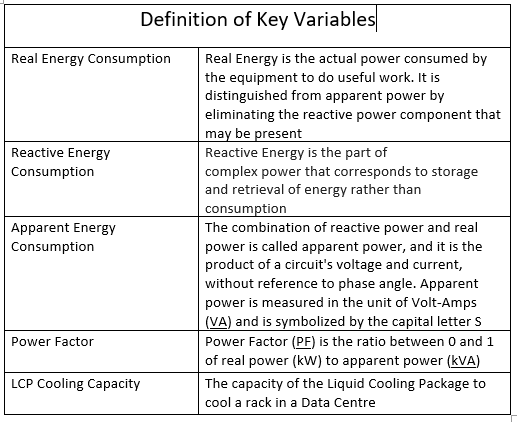
\includegraphics[scale=0.75]{key_variables}
\end{figure} 


\section{Detailed Correlation Analysis Results}
\label{sec:[Correlation Analysis Results]}
This section provides the detailed correlation analysis as outlined in section \ref{subsubsec:[Analyse Correlations]}





\begin{figure}[h]
  \caption{The Detailed Correlation Analysis Results - section 1}
  \label{fig:Correlation_Analysis_1}
  \centering
    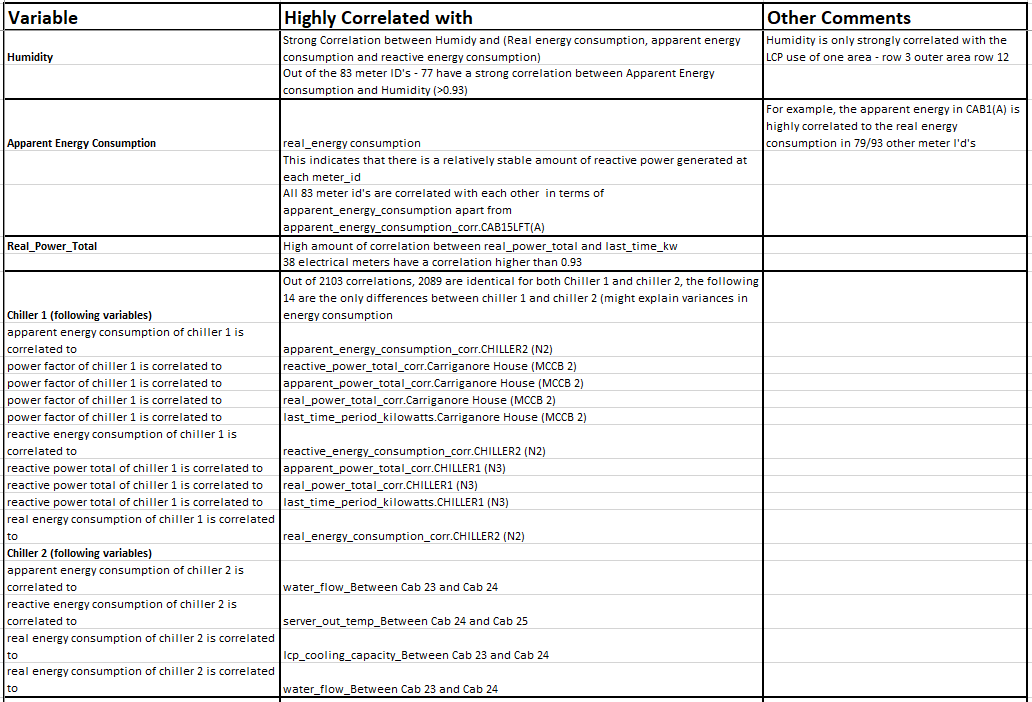
\includegraphics[scale=0.50]{Correlation_Analysis_1}
\end{figure} 

\begin{figure}[h]
  \caption{The Detailed Correlation Analysis Results - section 2}
  \label{fig:Correlation_Analysis_2}
  \centering
    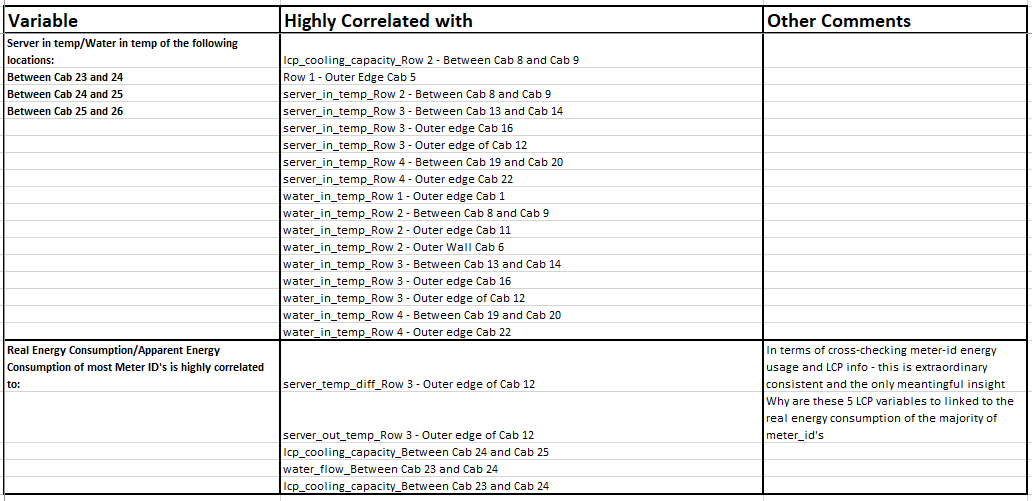
\includegraphics[scale=0.50]{Correlation_Analysis_2}
\end{figure} 



\end{document}
